\documentclass[tikz, margin=5mm]{standalone}
\usepackage{sfmath}
\usepackage{amsmath}
\usepackage[scaled]{helvet}
\renewcommand\familydefault{\sfdefault}
\usepackage[T1]{fontenc}

\definecolor{mycolour}{RGB}{239,131,118}
\usetikzlibrary{fit,positioning,arrows.meta}

\begin{document}
\begin{tikzpicture}[
   font=\sffamily,
   arrow/.style={->,mycolour,line width=1mm},
   axis/.style={->,line width=.75mm},
   box/.style={mycolour,rounded corners=1mm, line width=.5mm},
   circlenode/.style={fill=mycolour, color=mycolour, line width=.75mm}
]

% Input
\node[align=center, text width=4cm] at (0, 6) {\large Spectrogram };
\node[inner sep=0pt] at (0,0) {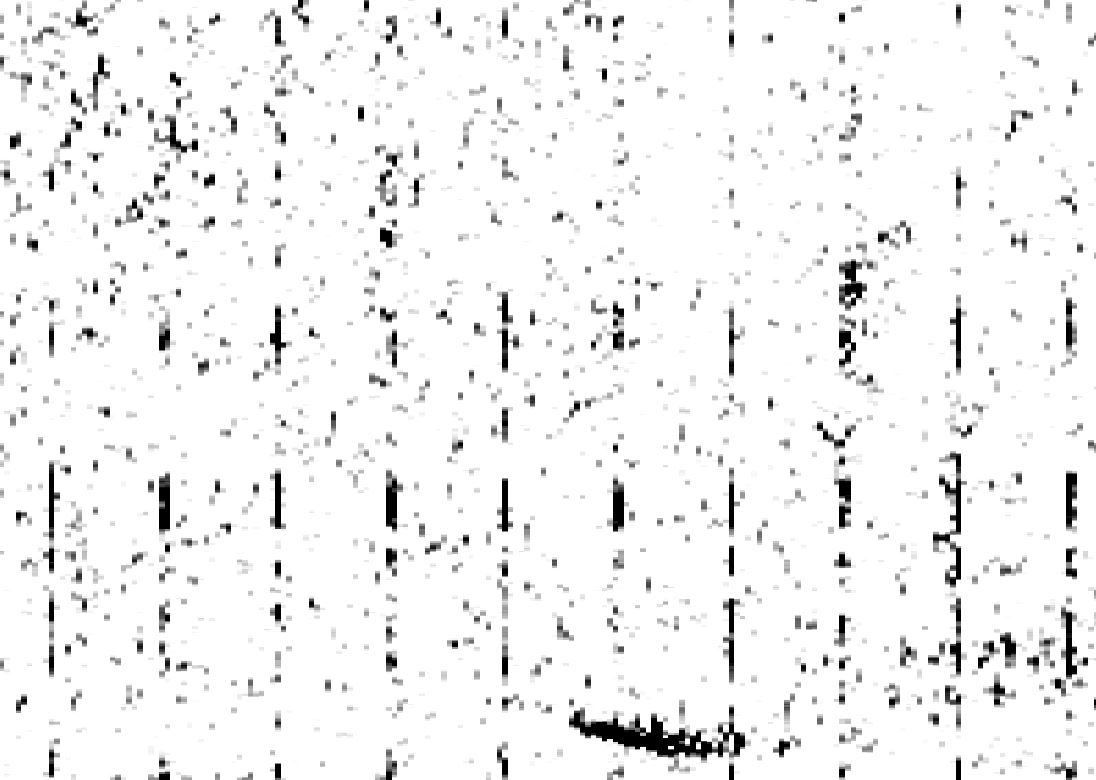
\includegraphics[width=10cm, height=10cm]{images/pamlab_example}};
\draw[axis] (-5,-4.985) -- (-5,5.3) node[midway, above, rotate=90] {\huge Freq (Hz)};
\draw[axis] (-5,-4.95) -- (5.3,-5) node[midway, below] {\huge Time (s)};;

% Robot
\node[inner sep=0pt] at (8,2) {
\includegraphics[height=2cm]{images/robot_emoji.png}};
\draw[arrow, line width=.75mm] (7,1) -- (1.75,-4) node{};

% Annotation Box
\pgfmathsetmacro{\cubex}{1.5}
\pgfmathsetmacro{\cubey}{.75}
\draw[box, line width=.75mm] (1.65,-4,0) -- ++(-\cubex,0,0) -- ++(0,-\cubey,0) -- ++(\cubex,0,0) -- cycle;
\draw[arrow, line width=.75mm] (1.65,-4.25) -- (7,-2.25) node{};

% Female Technologist
\node[inner sep=0pt] at (8,-2) {
\includegraphics[height=2cm]{images/technologist_emoji.png}};

\end{tikzpicture}
\end{document}
